%!TEX root = ../thesis.tex
\ifpdf
    \graphicspath{{Chapter4/Figs/Vector/}{Chapter4/Figs/PDF/}{Chapter4/Figs/}}
\else
    \graphicspath{{Chapter4/Figs/Raster/}{Chapter4/Figs/}}
\fi



\chapter{Deep Neural Networks as Point Estimates for Deep Gaussian Processes}
\label{chapter:dnn-as-point-estimate-for-dgps}

Neural networks (NNs) and Gaussian processes (GPs) are complementary in their strengths and weaknesses. Having a better understanding of their relationship comes with the promise to make each method benefit from the strengths of the other. In this chapter, we establish an equivalence between the forward passes of neural networks and the posterior of deep sparse Gaussian process models. The theory we develop builds upon the RKHS presented in \cref{chapter:vish} and is based on interpreting activation functions as interdomain inducing features through a rigorous analysis of the interplay between activation functions and kernels. This results in models that can either be seen as neural networks with improved uncertainty prediction or deep Gaussian processes with increased prediction accuracy. In \cref{section:dnn-for-dgps:related-work} we first give a brief overview of the rich literature on Bayesian treatments of NNs and how this gives rise to (deep) GPs. In \cref{section:dgps} we then formally introduce Deep Gaussian processes (DGPs) and highlight the close similarly between NNs and the posterior of sparse DGPs. In \cref{sec:dnn-for-dgps:model} we present our \emph{activated} inducing variables for which the resulting GP basis functions match traditional neural network activation, which gives rise to the equivalence between DGPs and NNs.  Our claims are supported by experimental results on the UCI repository benchmarks and a series of image classification tasks in \cref{section:dnn-for-dgps:experiments}.

\section{Related Work}
\label{section:dnn-for-dgps:related-work}
Many different relationships between GPs and NNs have been established over the years. These relationships mainly arise from Bayesian approaches to neural networks. %, which quantify the uncertainty about the function that is being learned, which is useful for robust prediction and decision making. 
Finding the posterior distribution on neural network weights is challenging, as closed-form expressions do not exist. As a consequence, developing accurate approximations has been a key goal since the earliest works on Bayesian NNs \citep{mackay1992practical}.
While investigating single-layer NN posteriors, \citet{neal1996bayesian} noticed that randomly initialised NNs converged to a \emph{Gaussian process} (GP) in the limit of infinite width.
Like NNs, GPs represent functions, although they do not do so through weights. Instead, GPs specify function values at observed points, and a kernel which describes how function values at different locations influence each other.

This relationship was of significant practical interest, as the mathematical properties of GPs could \textbf{1)} represent highly flexible NNs with \emph{infinite} weights, and \textbf{2)} perform Bayesian inference without approximations.
This combination was highly successful for providing accurate predictions with reliable uncertainty estimates \citep{williams1996gaussian,rasmussen1997evaluation}.
To obtain models with various properties, GP analogues were found for infinitely-wide networks with various activation functions \citep{williams1998computation,mackay1998introgp} including the ReLU \citep{cho2009kernel}. More recently, \citet{Meronen2020} investigated the relationship in the opposite direction, by deriving activation functions such that the infinite width limit converges to a given GP prior.

Since the growth of modern deep learning, relationships have also been established between infinitely wide \emph{deep} networks and GPs \citep{matthews2018gaussian,lee2018dnnlimit,yang2019wide}. Given these relationships, one may wonder whether GPs can supersede NNs, particularly given the convenience of Bayesian inference in them. Empirically though, finite NNs outperform their GP analogues \citep{lee2018dnnlimit,garriga2018deep,novak2018bayesian} on high-dimensional tasks such as images. \citet{mackay1998introgp} explained this by noting that NNs lose their ability to learn features in the infinite limit, since every GP can be represented as a single-layer NN, with \emph{fixed} features \citep{mercer1909,rasmussen2006weightfunc}.
This observation justifies the effort of performing approximate Baysian inference in \emph{finite} deep networks, so both feature learning and uncertainty can be obtained. Renewed effort in Bayesian training procedures has focussed on computationally scalable techniques that take advantage of modern large datasets, and have provided usable uncertainty estimates \citep[e.g.,][]{Kingma2015local,blundell2015,Gal2016dropout,louizos2016}.

However, questions remain about the accuracy of these approximations. %One insight is given by the relationship between the accuracy of uncertainty estimates, and estimates of the marginal likelihood, which is particularly clear in variational inference \citep{blei2017variational}. 
For accurate Bayesian inference, marginal likelihoods are expected to be usable for hyperparameter selection \citep{mackay1992bmc,mackay2003information}. For most current approximations, there is either no positive or explicitly negative \citep{blundell2015} evidence for this holding, although recent approaches do seem to provide usable estimates \citep{ober2020global,immer2021marglik}.

DGPs \citep{Damianou2013} provide an alternative approach to deep NNs, which use GP layers instead of weight-based layers, in order to take advantage of the improved uncertainty estimates afforded by having an infinite number of weights. % As training procedures developed, strong similarities to NNs have been uncovered \citep{hensman2014nested,bui2019dgpep,salimbeni2017doubly}. 
The DGP representation is particularly promising because both early and recent work \citep{Damianou2013,damianou2015thesis,Dutordoir2020convolutional} shows that marginal likelihood estimates are usable for hyperparmeter selection, which indicates accurate inference. However, currently scalability and optimisation issues hinder widespread use. 


% \citet{mackay1992practical,mackay1992bmc} noted very early that the Bayesian treatment of neural networks had large potential. To start, it can help to quantify estimates of the error bars on the network outputs, but it can also provide an objective that can be used for the comparison of alternative network architectures. The reality, however, was that Bayesian inference in neural networks was --and still is-- challenging, and in practice one has to resort to either crude approximations (e.g., Laplace approximation \citep{MacKay1998laplace}) or lengthy computations (e.g., Markov Chain Monte Carlo \citep{neal1992bayesian}).

% Building on the foundational work of MacKay, and driven by the amazing successes of large deterministic deep neural networks (DNNs), the literature has seen an upspring in the development of more scalable methods to perform approximate Bayesian inference in DNNs \citep{blundell2015,Kingma2015local,Gal2016dropout}. However, it remains challenging to encode prior assumptions on functions through distributions on weights and the large number of parameters to be estimated makes it computationally prohibitive. Furthermore, the strong approximations used both during modelling and inference make it unclear to what extent these models approximate the true posterior distribution \citep{hron2017variational, foong2019expressiveness}. They also do not deliver on an important promise of Bayesian methods: an approximate marginal likelihood objective that can be used for automatic model selection and hyperparameter learning. A different approach may thus be necessary to unlock the Bayesian benefits in deep learning.

% \citet{neal1996bayesian} showed that for infinitely wide single-layer BNNs the distribution over the non-linear functions are given by Gaussian processes. \citet{williams1998computation,cho2009kernel} extended this theory and derived the kernel corresponding to an infinite-width BNN with Sigmoidal and ReLU activation function, respectively. The beauty of this connection is that performing Bayesian inference in the corresponding GP model can be done exactly and analytically -- all in a single elegant framework \citep{rasmussen2006}. Since, various approximations to the exact GP framework have been developed to allow for non-Gaussian likelihoods \citep{kuss2005assessing,hensman2013}, large datasets \citep{hensman2015scalable, wang2019exact}, and even neural network like structures such as convolutions \citep{vanderwilk2017conv}. Crucially, the approximations to the marginal likelihood still enable the main Bayesian benefits: model uncertainty and learning model hyperparameters (e.g., \citep{vanderwilk2018invariances,Dutordoir2020convolutional}).

% More recently, \citet{matthews2018gaussian} discovered the equivalence between \emph{deep} (i.e. multi-layer) BNNs and GPs. This has led to the development of deep (fully connected and convolutional) neural network kernels for GPs (NN-GPs). Interestingly, the performance of the non-Bayesian neural nets significantly outperforms the corresponding GPs \citep{garriga2018deep,novak2018bayesian}. The discrepancy hints at the fact that these single-layer GPs, even when configured with very expressive DNN equivalent kernels, are missing a crucial component: the ability to learn feature representations from the data.
% % From James' Variationally compressed DGPs: ``Both Neal [1996] and MacKay [1998] pointed out some of the limitations of priors that ensure joint Gaussianity across observations and this has inspired work in moving beyond Gaussian processes"

% Deep Gaussian processes \citep[DGPs]{Damianou2013} are an interesting avenue to tackle these challenges. They are built by hierarchically stacking GPs on top of each other, which enables the learning of more powerful representations through compositional features. Moreover, their Bayesian approximations in function-space seem to be of higher quality than those of weight-space BNNs, e.g.~as supported by the successful use of marginal likelihood estimates for hyperparameter learning \citep{Damianou2013}.
% % DGPs have been shown to be accurate and robust in the low-data regime, to allow for automatic model selection and hyperparameter learning, and to exhibit accurate predictive uncertainty \citep{Damianou2013, salimbeni2017doubly,Dutordoir2020convolutional}.

% While promising, DGPs have struggled for relevance in applications due to the challenges and cost associated with Bayesian inference. Training DGPs is computationally expensive and requires very careful setting of the parameters. Furthermore, the hierarchical prior induced by naively stacking stationary kernels gives rise to pathological, ``collapsed'' samples \citet{duvenaud2014avoiding}. Considerable progress for scalable inference in DGPs was made by \citet{hensman2014nested, salimbeni2017doubly}, who derived stochastic variational lower bounds. The formulation of these bounds closely resembles the computations of training a feed-forward neural network with regularisation terms, and has greatly inspired this work.

% Building on \citet{salimbeni2017doubly} and to further improve the scalability of DGPs, \citet{cutajar2017random} used a Random Fourier Feature \citep[RFF]{rahimi2008random} approximation of the kernel. While successful, this approach introduces an approximation in both the prior and the posterior of the model. More recently, \citet{rudner2020inter} proposed Fourier features of the Mat\'ern RKHS, following \citet[Variational Fourier Features (VFF)]{hensman2017variational}, to build inter-domain DGPs. Like for single layer VFF models, this approach can lead to faster training and improved performance, but is only computationally feasible for data of dimension one or two. In parallel with our work, \citet{sun2021neural} explored the idea of using single-layer neural networks to parameterise inducing points in shallow GPs. Similar to this paper, their method makes use of the spherical harmonic decomposition of a kernel. However, their works differs in the fact that they focus on shallow GPs, on bounded inducing functions (e.g.,  $\textrm{erf}$), and directly use the Nystr\"om approximation to approximate the model's uncertainty estimates rather than the ELBO to learn the variational parameters.

% The analysis of (Bayesian) neural networks has led to several probabilistic models: NN-GPs, GPs and DGPs. In this work, however, rather than focusing on the \emph{prior} induced by these equivalent models, the emphasis lies on the connection between the DGP \emph{posterior} and the DNN. This has received much less attention in the literature, though we argue it is a more interesting regime to study. The connection between GP piors and neural nets is established only in the infinite limit of the number of hidden units. The sparse posterior DGP, on the contrary, is built out of a finite set of basis functions and can thus immediately be connected to finite-width neural networks --- in this paper we connect both models in their modus operandi.

% We formulate a DGP configuration for which the approximate posterior mean has the same mathematical structure as a deep neural network with fully connected layers and non-linear activation functions. We can use this unification to train the DGP like a neural network which allow us to leverage all the great research in this area for DGP inference. Furthermore, this connection between DGPs posteriors and DNNs highlights the great potential of DGPs as a model for learning powerful representations from data while being fully Bayesian.

\section{Deep Gaussian Processes}
\label{section:dgps}

GPs are often used as priors over functions in supervised learning, as for Gaussian likelihoods the posterior $f \given \mathcal{D}$ given a dataset $\mathcal D = \{x_i \in \Reals^d, y_i \in \Reals\}_{i=1}^N$ is tractable (see \cref{sec:gp-exact-inference}). Surprisingly diverse properties of the GP prior can be specified by the kernel \citep{rasmussen2006,duvenaud2013structure,wilson2013gaussian,ginsbourger2013kernels,vanderwilk2018invariances}, although many problems require the flexible feature learning that deep NNs provide. DGPs \citep{Damianou2013} propose to solve this in a fully Bayesian way by composing several layers of simple GP priors,
\begin{equation}
    \mathcal{F} = f_L \circ \ldots \circ f_2 \circ f_1\qquad\text{where}\qquad
        f_\ell \sim \GP\big(0, k_\ell\big).
\end{equation}

Inference in DGPs is challenging as the composition is no longer a GP, leading to an intractable posterior $\mathcal{F} \given \mathcal{D}$.  Various approximations have been developed over the years \citep{Damianou2013,hensman2014nested,bui2019dgpep,havasi2018inference}. We follow the variational approach by \citet{salimbeni2017doubly} due to its similarity to backpropagation in NNs. They use an approximate posterior consisting of an independent sparse GP for each layer. Each sparse GP is constructed by conditioning the prior on $M$ inducing variables \citep{titsias2009,hensman2013,matthews16}, commonly function values $\vu_\ell = \{u^m_\ell = f_\ell(w_\ell^m)\}_{m=1}^M$, and then specifying their marginal distribution as $q(\vu_\ell) = \NormDist{\vm_\ell, \MS_\ell}$. This results in the approximate posterior process:
\begin{equation}
\label{eq:qf-dgp}
     q(f_\ell(x)) = \GP\Big(\kul^\top(x) \Kulul^{-1}\vm_\ell,\ \ k_\ell(x, x') -  \kul^\top(x) \Kulul^{-1} (\Kulul + \MS_\ell)\Kulul^{-1} \kul(x)\Big).
\end{equation}
%
% \begin{equation}
%     \label{eq:qf}
%     q(f) = \GP\Big(\kux^\top \Kuu^{-1}\vm,\ \ k(\cdot, \cdot) -  \kux^\top \Kuu^{-1} (\Kuu + \MS)\Kuu^{-1} \kux\Big).
%   \end{equation}

% where $\vb_\ell = \Cuuell^{-1} \vmu_\ell$ (or $\MB_\ell$ in the multi-output case) and $\cuell(\cdot) = \Cov(f_\ell(\cdot), \vu_\ell)$ and $\Cuuell = \Cov(\vu_\ell, \vu_\ell)$. 
%
%  Subsequently, we will be dealing with multi-output GPs then for each output $p$ we have $\vb_p = \Cuu^{-1} \vmu_p$ with $\vmu_p$ and $\MSigma_p$ the mean and covariance of the inducing outputs, $u_{m, p} = f_p(\vz_m)$ and $q(\vu_p) = \NormDist{\vmu_p, \MSigma_p}$. We collect $\{\vb_p \in \Reals^M \}_{p=1}^P$ as the columns of the matrix $\MB \in \Reals^{M \times P}$.
%
The variational parameters $\vm_\ell \in \Reals^M$ and $\MS_\ell \in \Reals^{M \times M}$ are selected by reducing the Kullback-Leibler (KL) divergence from the variational distribution to the true posterior. This is equivalent to maximising the Evidence Lower BOund (ELBO). Taking the evaluations of the GP as $\vh_{:, \ell} = f_\ell(\vh_{:, \ell-1})$, the ELBO becomes \citep{salimbeni2017doubly}:
\begin{equation}
\label{eq:dgp-elbo}
\log p(\vy) \ge \sum\nolimits_i \Exp{q(h_{i, L})}{\log p(y_i \given h_{i, L})} - \sum\nolimits_{\ell} \KL{q(\vu_\ell)}{p(\vu_\ell)}.
\end{equation}

\begin{figure}[t]
    \centering
    \begin{subfigure}[b]{0.48\textwidth}
         \centering
        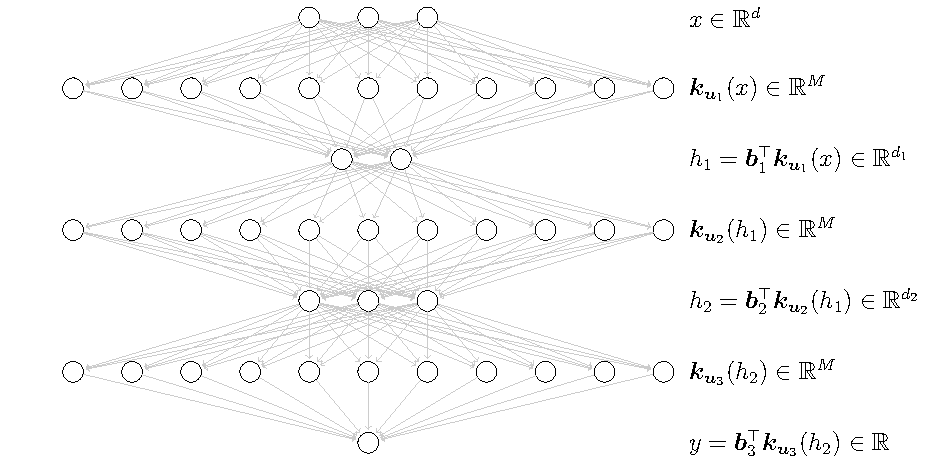
\includegraphics[width=\textwidth]{dgp_v2}
        \caption{Deep Gaussian process posterior}
        \label{fig:visual-dgp}
     \end{subfigure}
     \hfill
     \begin{subfigure}[b]{0.51\textwidth}
         \centering
        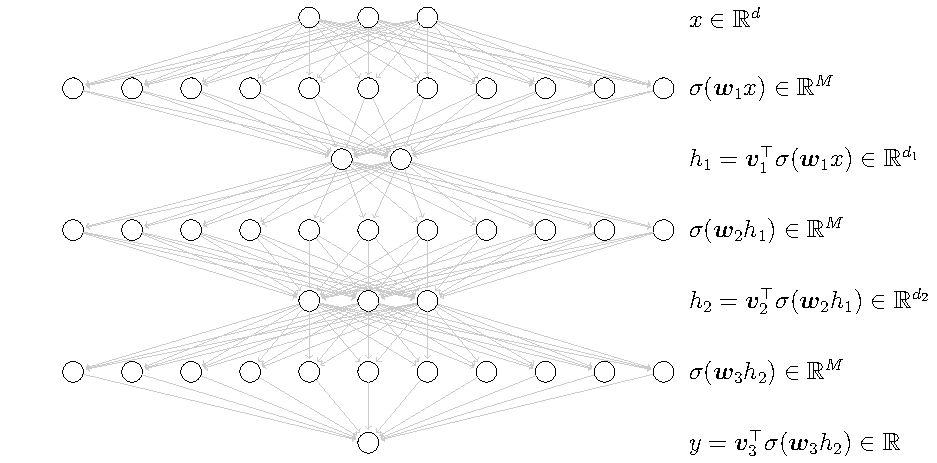
\includegraphics[width=\textwidth]{nn_v2}
         \caption{Fully-connected deep neural network}
         \label{fig:visual-nn}
     \end{subfigure}
    \caption{Forward pass through a DGP \textbf{(a)} and a DNN \textbf{b}. By matching basis functions $\kul(x)$ with $\sigma(\vw_\ell x)$ and weights $\bm{b}_\ell$ with $\bm{v}_\ell$ we obtain an equivalence between both models.} % Comparison between a DGP \textbf{(a)} and a DNN \textbf{(b)}. The goal is to design basis functions $\vc_{\vu}(\cdot)$ for the DGP that match to the activation functions $\sigma(\MW\,\cdot)$ used in the DNN.}
    \label{fig:visual}
\end{figure}

\subsection{Connection to Deep Neural Networks}
Investigating \cref{eq:qf-dgp}, it is worth noting that the posterior $q(f_\ell)$'s variance takes into account the infinite degrees of freedom from the prior; making predictions with an infinite amount of basis functions. The mean, on the contrary, has a finite numbers of parameters and can straightforwardly be re-written as a linear model with $M$ basis functions of the form $\kul(x) = \Cov(\vu_\ell, f_\ell(x))$:
\begin{equation}
    \label{eq:mean-qf}
    \Exp{f_\ell}{q(f_\ell(x))} = \bm{b}_\ell^\top \kul(x) \quad \text{where} \quad \bm{b}_\ell = \Kulul^{-1} \vm_\ell \in \Reals^M
\end{equation}
The mean of a layer in DGP is therefore ``not that different'' from a fully-connected layer in a neural network (NN-FCL), which admits the following structure
\begin{equation}
    \label{eq:fcn}
    \text{NN-FCL}_\ell(x) = \bm{v}_\ell\transpose \sigma(\bm{w}_\ell\,x),
\end{equation}
where $\sigma$ is the non-linear activations function (e.g., ReLU), $\bm{w}_\ell \in \Reals^{M \times d}$ and $\bm{v}_\ell \in \Reals^{M \times d_\ell}$ are the pre-activation and output weights, respectively. Looking at the resemblance between \cref{eq:mean-qf} and \cref{eq:fcn}, if we are able to formulate an inducing variable that makes the covariance $\kul(x)$ the same as a neural net activation function $\sigma(\bm{w}_\ell\,x)$, we will have a formal mathematical equivalence between the mean of GP layer in a DGP and a fully-connected neural network layer, that is $\ExpSymb[q(f_\ell(x))] = \text{NN-FCL}_\ell(x)$. By stacking many of these layers we obtain an equivalence between the forward pass in a DGP and a DNN, as visualised in \cref{fig:visual}.

In the next section we design the interdomain inducing variable for which the covariance will match the neural network activation function. This is the main contributions of this chapter. 


\section{Gaussian Process Layers with Activated Inducing Variables}
\label{sec:dnn-for-dgps:model}

Building on the exposition of zonal kernel RKHSs (\cref{sec:rkhs-dotproduct-kernels}) and interdomain inducing variables (\cref{section:interdomain-inducing-variables}) we can summarise our approach succinctly: we consider DGP models with GP layers that have an Arc Cosine kernel and Variational Fourier Feature style inducing variables $u_m = \langle f, {g}_m \rangle_\rkhs$ \citep{hensman2017variational}. We then choose inducing functions $g_m$ that have the same shape as neural network activation functions (\cref{sec:inducing-function}). Thanks to the reproducing property of the RKHS this yields basis functions $\kulx$ for the GP layers that correspond to activation functions (\cref{sec:relu-inducing-variables}), and thus to a DGP whose forward pass can be interpreted as a classic feed forward neural network. \Cref{sec:zonal-kernels-and-rkhs} covers the mathematical intricacies associated with the construction described above.

%%%%%%%%%%%%%%%%%%%%%%%%%%%%%%%%%%%%%%%%%%%%%%%%%%%%%%%%%%%%%%%%%%%%%%%%%
\subsection{Activated Inducing Functions}
\label{sec:inducing-function}

We consider the RKHS of the first-order Arc Cosine kernel as discussed in \cref{sec:rkhs-dotproduct-kernels}, which has a form
The RKHS of the Arc Cosine kernel consists solely of functions that are equal to zero at the origin, i.e. $\forall f \in \rkhs: f(\bm{0}) = 0$. 
%This is not a desired property for many datasets and a common approach
To circumvent this problem we artificially increase the input space dimension by concatenating a constant to each input vector. In other words, the data space is embedded in a larger space with an offset such that it does not contain the origin anymore. This is analogous to the bias unit in multi-layer perceptron (MLP) layers in neural networks. For convenience we will denote by $(d-1)$ the dimension of the original data space (i.e. the number of input variables), and by $d$ the dimension of the extended space on which the Arc Cosine kernel is defined.

\begin{figure}[t]
    \centering
     \begin{subfigure}[b]{0.49\textwidth}
         \centering
        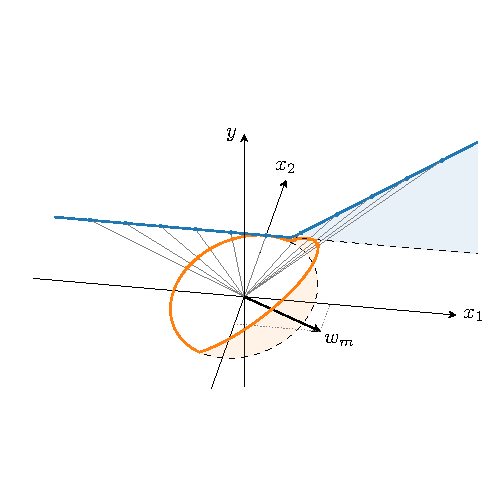
\includegraphics[clip, trim=0cm 1.8cm 0cm 1.6cm, width=\textwidth]{relu_mapping}
        %  \caption{$g_m(\vx) = \norm{\vw_m} \norm{\vx} \max\left(0, \frac{\vw_m^\top \vx}{\norm{\vw_m} \norm{\vx}}\right)$}
        \caption{ReLU: $\sigma(t) = \max(0, t)$}
         \label{fig:projection:relu}
     \end{subfigure}
     \hfill
     \begin{subfigure}[b]{0.49\textwidth}
         \centering
        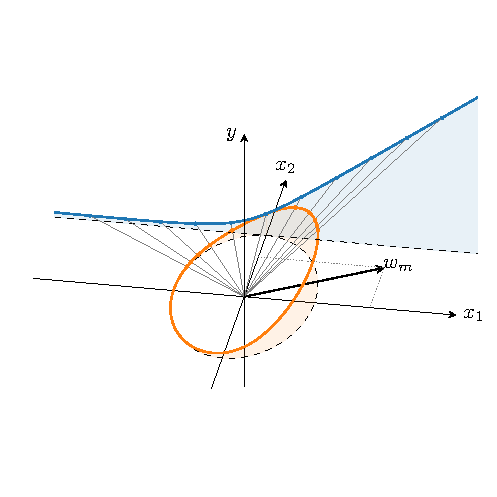
\includegraphics[clip, trim=0cm 1.8cm 0cm 1.6cm, width=\textwidth]{softplus_mapping}
        %  \caption{$g_m(\vx) = \norm{\vw_m}\norm{\vx} \left(\log(1 + \exp(\frac{3 \vw_m^\top \vx}{\norm{\vw_m} \norm{\vx}})) - c\right) $}
        \caption{Softplus: $\sigma(t) = \log(1 + \exp(3\,t))$}
         \label{fig:projection:softplus}
     \end{subfigure}
   \caption{Activated inducing function ${g}_m(x) = \norm{x}\,\norm{w_m}\, \sigma\left( w_m^\top x \, / \, \norm{w_m}\,\norm{x}\right)$ where $\sigma$ correspond to the ReLU \textbf{(a)} and Softplus \textbf{(b)}. Although the input domain is $\Reals^2$ we only plot the value of the function on the unit circle $\sphere^1$ (orange), and on the subspace that has an offset of $1$ in the $x_2$ direction (blue). The linear radial component of ${g}_m$ creates a one-to-one mapping between the blue curve and the upper half of the orange one.}%We observe that for these slices the functions correspond to the ReLU and Softplus neural network activation functions, respectively.}
   \label{fig:projection}
\end{figure}

The inducing functions $g_m$ play an important role because they determine the shape of the SVGP's basis functions. Ideally they should be defined such that their restriction to the $(d - 1)$-dimensional original data space matches classic activation functions, such as the ReLU or the Softplus, exactly. However, this results in an angular component for $g_m$ that is not necessarily zonal. Since this property will be important later on, we favour the following alternative definition that enforces zonality:
\begin{equation}
\label{eq:def-inducing-function}
    g_m: \Reals^d \rightarrow \Reals,\qquad x \mapsto \norm{x}\,\norm{w_m}\, \sigma\left(\frac{w_m^\top x}{\norm{w_m}\,\norm{x}}\right), 
\end{equation}
with $w_m \in \Reals^d$ a parameter, and $\sigma: [-1, 1] \rightarrow \Reals$ the function that determines the value of $g_m$ on the unit hypersphere. In \cref{fig:projection}, we show that choosing $\sigma$ to be a ReLU ($\sigma(t) = \max(0, t)$) or a Softplus ($\sigma(t) = \log(1 + \exp(3\,t))$) activation function leads to inducing functions that closely resemble the classic ReLU and Softplus on the data space. In the specific case of the ReLU it can actually be shown that the match is exact. In both cases, the parameter $w_m \in \Reals^d$ determines the orientation and slope of the activation function---they play the same role as the pre-activation weights in a NN.

The zonality that we enforced in \cref{eq:def-inducing-function} is particularly convenient when it comes to representing $g_m$ in the basis of the eigenfunctions of $\rkhs$, which is required for computing inner products. It indeed allows us to make use of the Funk-Hecke theorem (see \cref{app:sec:harmonics}) and to obtain
\begin{equation}
\begin{aligned}
\label{eq:fourier-decomposition-activation-functions-new}
    g_m(x) = \norm{x}\, \norm{w_m} \sum_{n=0}^\infty &\sum_{j=1}^{\dnumharmonicsforlevel}  \sigma_n \phi_{n, j}\left(\frac{w_m}{\norm{w_m}}\right)\, \phi_{n, j}\left(\frac{x}{\norm{x}}\right), \\
   & \text{where \quad} \sigma_{n} = 
   \frac{\omega_{d}}{C_n^{(\alpha)}(1)} \int_{-1}^1 \sigma(t)\,C_n^{(\alpha)}(t)\,(1 - t^2)^{\frac{d-3}{2}} \calcd{t}.
\end{aligned}
\end{equation}
Analytical expressions for $\sigma_n$ when $\sigma(t)=\max(0, t)$ are given in \cref{app:sec:compute-eigenvalues}.

% [Representing functions on the sphere as a truncated series \cref{fig:activation-functions}]




\subsection{Activated Interdomain Inducing Variables}
\label{sec:relu-inducing-variables}

We define our \emph{activated} interdomain inducing variables as
\begin{equation}
\label{eq:def-inducing-variable}
    u_m = \big\langle f, {g}_m \big\rangle_\rkhs.
\end{equation}
Since the GP samples do not belong to the RKHS there are mathematical subtleties associated with such a definition, which are detailed in \cref{sec:zonal-kernels-and-rkhs}. Assuming for now that they are indeed well defined, using these interdomain inducing variables as part of the SVGP framework requires access to two quantities: (i) their pairwise covariance, and (ii) the covariance between the GP and the inducing variables. The pairwise covariance, which is needed to populate $\Kuu$, is given by
\begin{equation}
\label{eq:kuu}
\Cov(u_{m}, u_{m'})
= \langle {g}_m, {g}_{m'} \rangle_\rkhs
= \sum_{\substack{n=0 \\ \lambda_n \neq 0}}^{\infty}
    \frac{\sigma_n^2}{\lambda_n}\,\frac{n + \alpha}{\alpha}\,C_n^{(\alpha)}\left(\frac{w_m^\top w_{m'}}{\norm{w_m}\,\norm{w_{m'}}}\right).  
\end{equation}
The above is obtained using the RKHS inner product from \cref{eq:RKHSinnerproduct}, the Fourier coefficients from \cref{eq:fourier-decomposition-activation-functions-new} and the addition theorem for spherical harmonics from \cref{app:sec:harmonics}. Secondly, the covariance between the GP and $u_m$, which determines $[k_u(x)]_m$, is given by:
\begin{equation}
\label{eq:kuf}
  \Cov(u_m, f(x)) = 
    % \Cov(u_m, f(\cdot)) = % \Exp{f}{f(\vx) \langle f(\cdot), g_m(\cdot) \rangle_\rkhs} = 
    \langle k(x, \cdot), {g}_m \rangle_\rkhs = {g}_m(x) 
    % = \norm{\vw_m} \norm{\vx} \sum_{n=0}^{\tilde{N}} \sigma_n \frac{n + \alpha}{\alpha}\,C_n^{(\alpha)}(\frac{\vw_m^\top \vx}{\norm{\vw_m} \norm{\vx}}).
\end{equation}
as a result of the reproducing property of the RKHS. It becomes clear that this procedure gives rise to basis functions that are equal to our inducing functions. By construction, these inducing functions match neural network activation functions in the data plane, as shown in \cref{fig:projection}. Using these inducing variables thus leads to an approximate posterior GP (\cref{eq:qf}) which has a mean that is equivalent to a fully-connected layer with a non-linear activation function (e.g.~ReLU, Softplus, Swish). 


%%%%%%%%%%%%%%%%%%%%%%%%%%%%%%%%%%%%%%%%%%%%%%%%%%%%%%%%%%%%%%%%%%%%%%%%%
\subsection{Analysis of the interplay between kernels and inducing functions}
\label{sec:zonal-kernels-and-rkhs}

In this section we describe the mathematical pitfalls that can be encountered \citep[e.g.,][]{sun2021neural} when defining new inducing variables of the form of \cref{eq:def-inducing-variable}, and how we address them. We discuss two problems: 1) the GP and the inducing function are not part of the RKHS, 2) the inducing functions are not expressive enough to explain the prior. Both problems manifest themselves in an approximation that is overly smooth and over-estimates the predictive variance.

\begin{figure}[t]
    \centering
    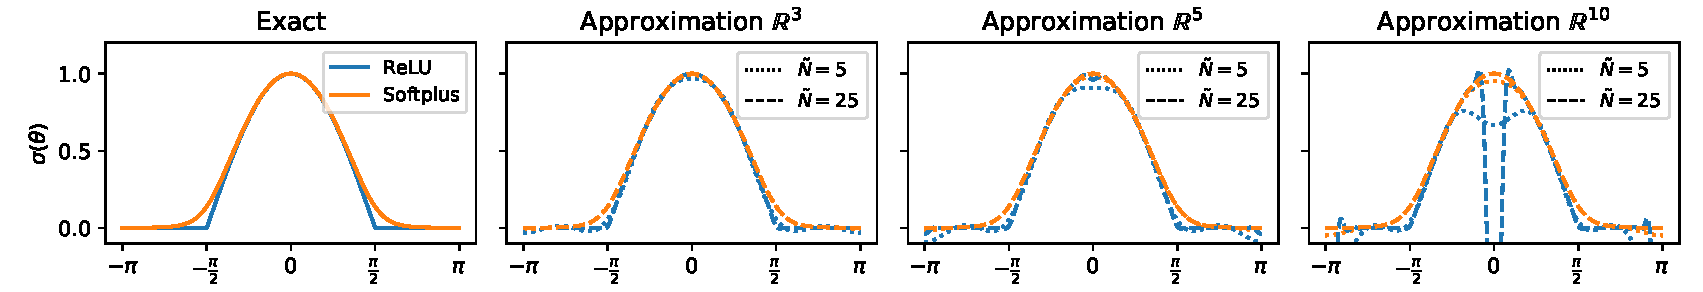
\includegraphics[width=\linewidth]{truncation_activations_circle}
    \caption{The exact ReLU and Softplus activation function and its approximation for different truncation levels and dimensions. These functions correspond to the orange function in \cref{fig:projection} plotted on a line rather than on the circle.}
    \label{fig:activation-functions}
\end{figure}

The Mercer representation of the kernel given in \cref{eq:mercer} implies that we have direct access to the Karhunen–Lo\`eve representation of the GP:
\begin{equation}
\label{eq:karhunen-loeve}
    f(\vx) =  \sum_{n=0}^\infty \sum_{j=1}^{\dnumharmonicsforlevel}  \xi_{n,j} \sqrt{\lambda_n} \norm{\vx} \sh_{n, j}\left(\frac{\vx}{\norm{\vx}}\right), \text{\quad where the } \xi_{n,j} \text{ are i.i.d. } \mathcal{N}(0, 1).
\end{equation}
Using this expression to compute the RKHS norm of a GP sample $f(\cdot)$ yields $\norm{f}^2 = \sum_{n, j} \xi_{n,j}^2$, which is a diverging series. This is a clear indication that the GP samples do not belong to the RKHS \citep{kanagawa2018gaussian}, and that expressions such as $\langle f(\cdot), g(\cdot) \rangle_{\rkhs}$ should be manipulated with care. According to the definition given in \cref{eq:RKHSinnerproduct}, the RKHS inner product is a series that converges if computed for any two elements  $g(\cdot), h(\cdot) \in \rkhs$. The inner product operator can however be extended to the case where one input lives in a space larger than $\rkhs$, provided that restrictions are introduced on the second input to guarantee the convergence of the series. In other words, even if the decay of the Fourier coefficients of $f(\cdot)$ is too slow to make it an element of \rkhs, if the Fourier coefficients of $g(\cdot)$ decay quickly enough for the series $\sum_{n,j} \xi_{n,j} g_{n,j}/ \sqrt{\lambda_n}$ to converge then $\langle f(\cdot), g(\cdot) \rangle_{\rkhs}$ is well defined.
%Though the theoretical setup in the previous paragraphs gives us an equivalence between a fully-connected neural network layer with a non-linear activation and the mean of an approximate SVGP, we need to proceed with caution to make sure that our method is mathematically sound, and practically useful. Indeed, since the GP samples do not belong to the RKHS, there are mathematical subtleties associated with manipulating expressions such as $\langle f(\cdot), g_m(\cdot) \rangle_{\rkhs}$ and attention must be paid to ensure this expression is meaningful. This is sometimes overlooked and can result in inducing variables with limited expressiveness, as it is the case in \citet{sun2021neural}.

%For the definition of the inducing variable (see~\cref{eq:fourier-decomposition-activation-functions-new}) to be valid a necessary condition is that $f(\cdot)$ and $g_m(\cdot)$ are both part of the RKHS. We already know that a GP sample does not belong to the RKHS \citep{kanagawa2018gaussian}, and, while we managed to write $g_m(\cdot)$ as a linear combination of the basis functions $\sh_{n, j}(\cdot)$ in \cref{eq:fourier-decomposition-activation-functions-new}, this does not guarantee its presence in $\rkhs$. This makes our inducing variables definition questionable. For the ReLU inducing function (i.e. $g_m(\cdot)$ with $\sigma(t) = \max(0,t)$ as in \cref{fig:projection:relu}), this concern is justified. Through the decay rate of $\sigma_n$, which is proportional to the square root of those of the corresponding Arc Cosine \citep{bach2017breaking,bietti2020deep}, it is easy to see that $\norm{g_m(\cdot)}_{\rkhs} > \infty$. This means that the ReLU inducing functions are not part of the first-order Arc Cosine RKHS ---reflecting the discontinuous nature of the function. Fortunately, by using smoother activation functions for $\sigma(t)$ (e.g.,~Softplus), for which the coefficients $\sigma_n$ decay faster than the eigenvalues of the kernel, the norm can be made finite and the activated inducing function part of the RKHS.

The above reasoning indicates that, for a given kernel $k(\cdot, \cdot)$, some activation functions $g_m(\cdot)$ will result in inducing variables $u_m = \langle f(\cdot), g_m(\cdot) \rangle_{\rkhs}$ that are well defined whereas other activation functions do not. For example, if we consider the case of the Arc Cosine kernel and the ReLU inducing function, the decay rate of $\sigma_n$ is proportional to the square root of $\lambda_n$~\citep{bach2017breaking,bietti2020deep}. This implies that the inner product series diverges and that this kernel and inducing variable cannot be used together. Alternatively, using smoother activation functions for $\sigma(t)$, such as the Softplus, results in a faster decay of the coefficients $\sigma_n$ and can guarantee that inducing variables are well defined.

An alternative to ensure the series convergence for any combination of kernel and activation function is to use a truncated approximation of the activation function $\tilde{g}_m(\cdot)$ where all the Fourier coefficients above a given level $\tilde N$ are set to zero, which basically turns the inner product series into a finite sum. % Making use of the addition theorem (see \cref{app:sec:harmonics}), this yields:
% \begin{equation}
%     \tilde{g}_m(\vx) = \norm{\vw_m} \norm{\vx} \sum_{n=0}^{\tilde{N}} \sigma_n \frac{n + \alpha}{\alpha}\,C_n^{(\alpha)}(\frac{\vw_m^\top \vx}{\norm{\vw_m} \norm{\vx}}).
% \end{equation}
\Cref{fig:activation-functions} shows how the true and truncated activation functions for the ReLU and Softplus compare. These correspond to the orange functions in \cref{fig:projection}, but are now plotted on a line. In the low to medium dimensional regime, we see that even for small truncation levels we approximate the ReLU and Softplus well. In higher dimensions this becomes more challenging for the ReLU. % and we notice high frequency variations near the boundary that are reminiscent of the Gibbs phenomenon in Fourier analysis. 

\paragraph{Unexpressive inducing variables through truncation (\cref{fig:trunc})} The main concern with this truncation approach, however, comes from elsewhere: the larger $\tilde N$ is, the closer $\tilde{g}_m(\cdot)$ is to $g_m(\cdot)$, but the larger $\norm{\tilde{g}_m(\cdot)}_{\rkhs}$ becomes (to the point where it may be arbitrarily large). Similarly to ridge regression where the norm acts as a regulariser, using inducing functions with a large norm in SVGP models comes with a penalty which enforces more smoothness in the approximate posterior and limits its expressiveness.
\Cref{fig:trunc} shows how the norm of our ReLU inducing functions grow in the RKHS. So by making $\tilde{N}$ larger such that we approximate the ReLU better, we incur a greater penalty in the ELBO for using them. This leads to unexpressive inducing variables, which can be seen by the growing predictive uncertainty. The Softplus, which is part of the RKHS, does not suffer from this.

\begin{figure}[t]
\centering
\begin{minipage}{.48\textwidth}
  \centering
  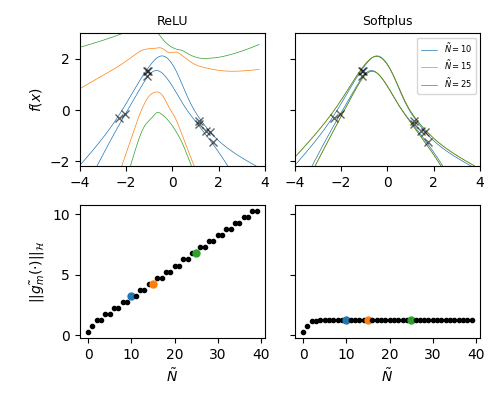
\includegraphics[width=\linewidth]{truncation_colors}
  \captionof{figure}{\textbf{Top:} Predictive variance an SVGP fit on a synthetic dataset using our ReLU (left) and Softplus (right) inducing variables for $\tilde{N}={\color{C0}10}, {\color{C1}15}$ and ${\color{C3}25}$. \textbf{Bottom:} the norm of the inducing function $\tilde{g}_m(\cdot)$ as a function of $\tilde{N}$.}
  \label{fig:trunc}
\end{minipage}\hfill
\begin{minipage}{.48\textwidth}
  \centering
  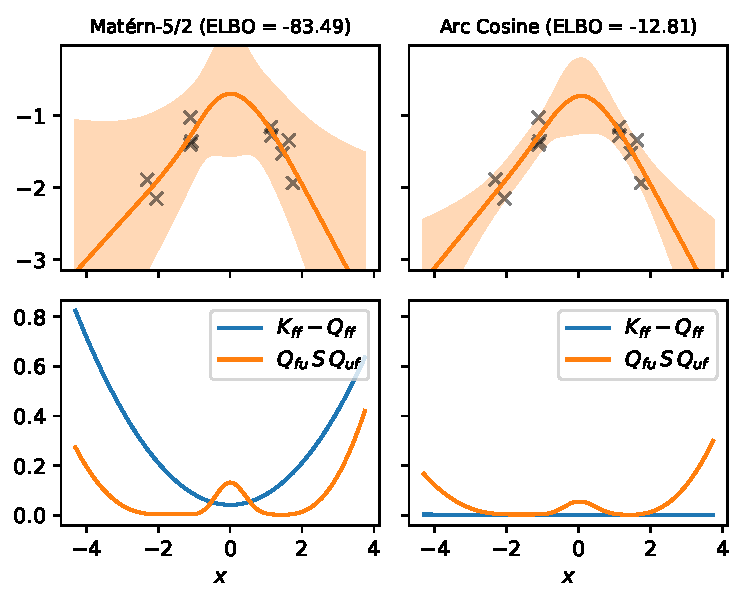
\includegraphics[width=\linewidth]{fits_and_variance_mat52_arccosine}
  \captionof{figure}{\textbf{Top:} Predictive mean and variance for an SVGP model using our Softplus inducing variables for the Mat\'ern-5/2 (left) and Arc Cosine (right) kernel. \textbf{Bottom:} The two terms that constitute the predictive variance.}
  \label{fig:matern-vs-arccosine}
\end{minipage}
\end{figure}

\paragraph{Unexpressive inducing variables through spectra mismatch (\cref{fig:matern-vs-arccosine})} Any stationary kernel whose inputs $\vx,\vx' \in \dsphere$ are restricted to the unit hypersphere is a zonal kernel (i.e., the kernel only depends on the dot-product). This means that we are not limited to only the Arc Cosine because we can replace the shape function in \cref{eq:arccosine} by any stationary kernel, and our approach would still hold. For example, we could use the Mat\'ern-5/2 shape function with $s_{\text{mat-5/2}}(t) = \left(1+{{{\sqrt {5}} t}}+{{5 t^{2}}/{3}}\right)\exp \left(-{{{\sqrt {5}} t}}\right)$. However, in \cref{fig:matern-vs-arccosine} we compare the fit of an SVGP model using a Mat\'ern-5/2 kernel (left) to a model using an Arc Cosine kernel (right). While both models use our Softplus inducing variables, we clearly observe that the Mat\'ern kernel gives rise to a worse posterior model (lower ELBO and an over-estimation of the variance). In what follows we explain why this is the case.

% In the bottom panel in \cref{fig:matern-vs-arccosine} we see that for the Mat\'ern-5/2, the Nystr\"om approximation $\Qff = \Cfu \Cuu^{-1} \Cfu^\top$ is unable to explain the prior $\Kff$, imposed by the kernel. This leads to the overestimation of the predictive variance in the top plot. The reason for this problem is the mismatch between the eigenvalues $\lambda_n$ (\cref{eq:compute-fourier-coefficients}) of the Mat\'ern and the Fourier coefficients $\sigma_n$ (\cref{eq:fourier-decomposition-activation-functions-new}) of the Softplus inducing function. As shown in \cref{fig:spectra}, the Mat\'ern kernel has a full spectrum (i.e., $\lambda_n \neq 0,\ \forall n \in \Naturals$), whereas the coefficients for the Softplus $\sigma_n$ are zero at levels $n=3, 5, 7,\cdots$. We are thus trying to approximate our prior kernel, containing all levels, by a set of functions that is missing many. This problem does not occur for the combination of Softplus (or ReLU) inducing functions and the Arc Cosine kernel (right-hand side) because their spectral decomposition match. In other words, the Arc Cosine kernel has zero coefficients for the same levels as our activated inducing functions. 



%%%%%%%%%%%%%%%%%%%%%%%%%%%%%%%%%%%%%%%%%%%%%%%%%%%%%%%%%%%%%%%%%%%%%% Experiments

\section{Experiments}
\label{section:dnn-for-dgps:experiments}

We have shown that that we can build SVGP models with basis functions that behave like neural net activations. This equivalence has the practical advantage that we can train the means of the GP layers in our DGP as if they are a neural network model --- making use of the great advances made by the deep learning community. Once the mean of the DGP is trained, we can further optimise the remaining model hyper- and variational parameters w.r.t. the ELBO, which is a more principled objective \citep{Fong2019On}. This approach allows us to exploit the benefit of both, the efficient training of the DNN in combination with the principled uncertainty estimate of the DGP. For all SVGP models we use the Arc Cosine kernel and inducing variables obtained with the Softplus activation (\cref{sec:inducing-function}) with $\tilde{N} = 20$, for the reasons explained in \cref{sec:zonal-kernels-and-rkhs}.

The aim of the experiments is to highlight that (i) our method leads to valid inducing variables, (ii) our initialisation improves DGPs in terms of accuracy, and (iii) we are able to improve on Dropout-based \citep{Gal2016dropout} neural networks in terms of calibrated uncertainty. 
%We show this on a wide range of problems.
We acknowledge that the NNs we benchmark against are the models for which we can build an equivalent DGP. While this leads to a fair comparison, it excludes recent improvements such as Transformer and Batch Norm layers.


% \begin{figure}[t]
%     \centering
%     \includegraphics[width=\linewidth]{figures/banana-M-ELBO.pdf}
%     \caption{Fits on the Banana binary classification dataset with growing number of inducing variables $M$. \textbf{left three panels:} In blue and orange we display the data. The model's $p(y \given \vx)$ is given as shades of grey. \textbf{right panel:} ELBO as a function of the number of inducing variables.}
%     \label{fig:banana}
% \end{figure}

% \paragraph{2D classification on Banana dataset} An attractive property of SVGPs (and DGPs) is that the objective is a lower bound on the log marginal likelihood, where the gap is the KL divergence between the true and approximate posterior. By increasing the number of inducing variables we make the approximate posterior richer, lowering the error, or equivalently, tighten the bound. In \cref{fig:banana} we verify this property for a single-layer SVGP model with our Softplus activated inducing variables and an Arc Cosine kernel. Given the small dataset size, we optimised the model's parameter using BFGS. This experiment validates that we designed valid inducing variables and that, as theory suggest, the ELBO improves with number of inducing variables.

% \begin{figure}[t]
%     \centering
%     \includegraphics[width=\linewidth]{figures/bananafull.pdf}
%     \caption{We compare the fit of a single-layer and three-layer DNN optimised using binary cross-entropy and it's equivalent DGP trained using the ELBO. The DNNs are very confident, even far away from the data. We used the DNNs to initialise the equivalent DGP posterior mean before optimising the ELBO, which in both situations leads to a model exhibiting more calibrated uncertainty.}
%     \label{fig:deep-banana}
% \end{figure}

% \paragraph{From Neural Network to Activated DGP} \Cref{fig:deep-banana} shows the difference in predictive probability $p(y \given \vx)$ for a DNN and our activated DGP, in the single-layer and three-layer case. We configure the models with a Softplus activation function and set the number of both inducing variables of the GP and hidden units of the DNN to 100. In this experiment, the first step is to optimise the DNN w.r.t. the binary cross-entropy objective, upon convergence we initialise the DGP with this solution and resume training of the DGP w.r.t. the ELBO. Especially in the single-layer case, we notice how the sharp edges from the NN are relaxed by the GP fit, and we see how the GP expresses uncertainty away from the data by letting $p(y \given \vx) \approx 0.5$. This is thanks to the ELBO, which balances both data fit and model complexity and simultaneously trains the uncertainty.

\subsection{Regression on UCI benchmarks}
We compare a suit of models on a range of regression problems. The important aspect is that we keep the model configuration and training procedure fixed across datasets. We use three-layered models with 128 inducing variables or hidden units. In each layer, the number of output heads is equal to the input dimensionality of the data. The Activated DGP (ADGP) and neural network approaches (Vanilla and Dropout) use Softplus activation functions. The Dropout model~\citep{Gal2016dropout} uses a rate of $0.1$ during train and test, and the Vanilla model is a deterministic neural network that uses the training MSE as the empirical variance during prediction.

The DGP and ADGP both use the Arc Cosine kernel. The main difference is that the DGP has standard inducing points $u_m = f(\vz_m)$, whereas ADGP makes use of our activated inducing variables $u_m = \langle f, g_m \rangle_\rkhs^{}$. The ADGP is trained in two steps: we first train the mean of the approximate posterior w.r.t. the MSE, and then optimise all parameters w.r.t. the ELBO.

In \cref{fig:uci} we see that in general our ADGP model is more accurate than its neural network initialisation (Vanilla model) in terms of RMSE. This is a result of the second stage of training in which we use the ELBO rather than the MSE, which is especially beneficial to prevent overfitting on the smaller datasets. When it comes to NLPD, ADGP shows improvements over its NN initialisation for 5 datasets out of 7 and consistently outperforms classic DGPs.

\begin{figure}
    \centering
    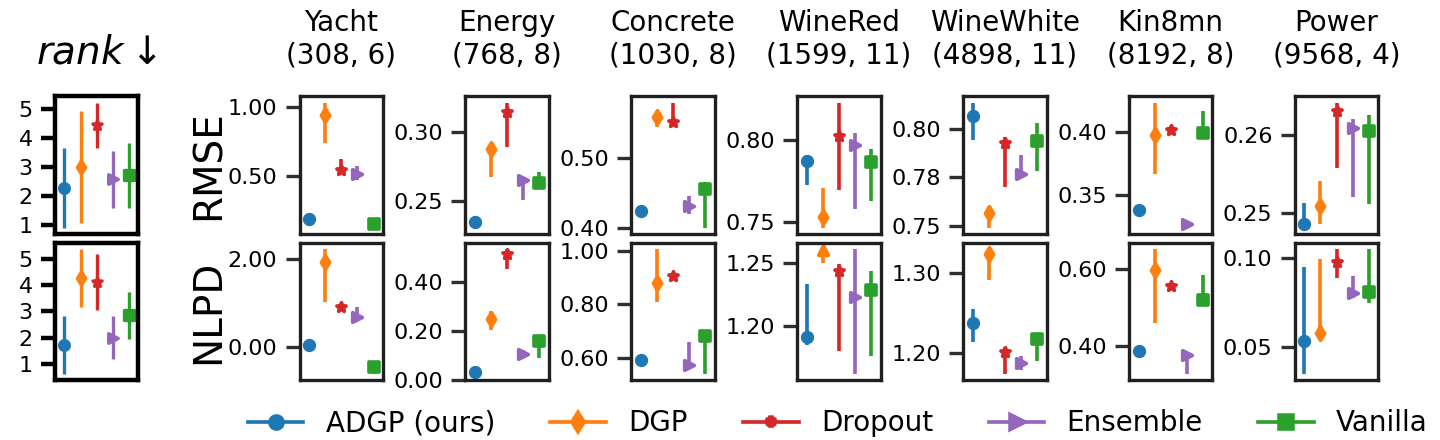
\includegraphics[width=\textwidth]{uci_small}
    \caption{UCI: Root Mean Squared Error (RMSE) and Negative Log Predictive Density (NLPD) with 25\% and 75\% quantile error bars based on 5 splits. Dataset size and dimension given in parentheses.}
    \label{fig:uci}
\end{figure}

\subsection{Large scale image classification}
% \label{sec:experiment:classification}
In this experiment we measure the performance of our models under dataset shifts \citep{Ovadia2019}. For MNIST and Fashion-MNIST the out-of-distribution (OOD) test sets consist of rotated digits --- from 0\textdegree (i.e. the original test set) to 180\textdegree. For CIFAR-10 we apply four different types of corruption to the test images with increasing intensity levels from 0 to 5. For MNIST and FASHION-MNIST the models consist of two convolutional and max-pooling layers, followed by two dense layers with 128 units and 10 output heads. The dense layers are either fully-connected neural network layers using a Softplus activation function (Vanilla and Dropout), or our Activated GP layers using the Arc Cosine kernel and Softplus inducing variables (ADGP). For the CIFAR-10 models, we use the residual convolutional layers from a ResNet~\citep{he2016deep} to extract useful features before passing them to our dense GP or NN layers. Details of the model architectures are given in \cref{app:sec:experiment}. As previously, the ADGP model is initialised to the solution of the Vanilla model, and training is then continued using the ELBO. In \cref{fig:image-classification} we observe that the models perform very similar in terms of prediction accuracy, but that ADGP better account for uncertainty as evidenced by the Test Log Likelihood metric.% (TLL) we see that the ADGP outperforms the NN approaches by quite a margin.

\begin{figure}[t]
    \centering   
    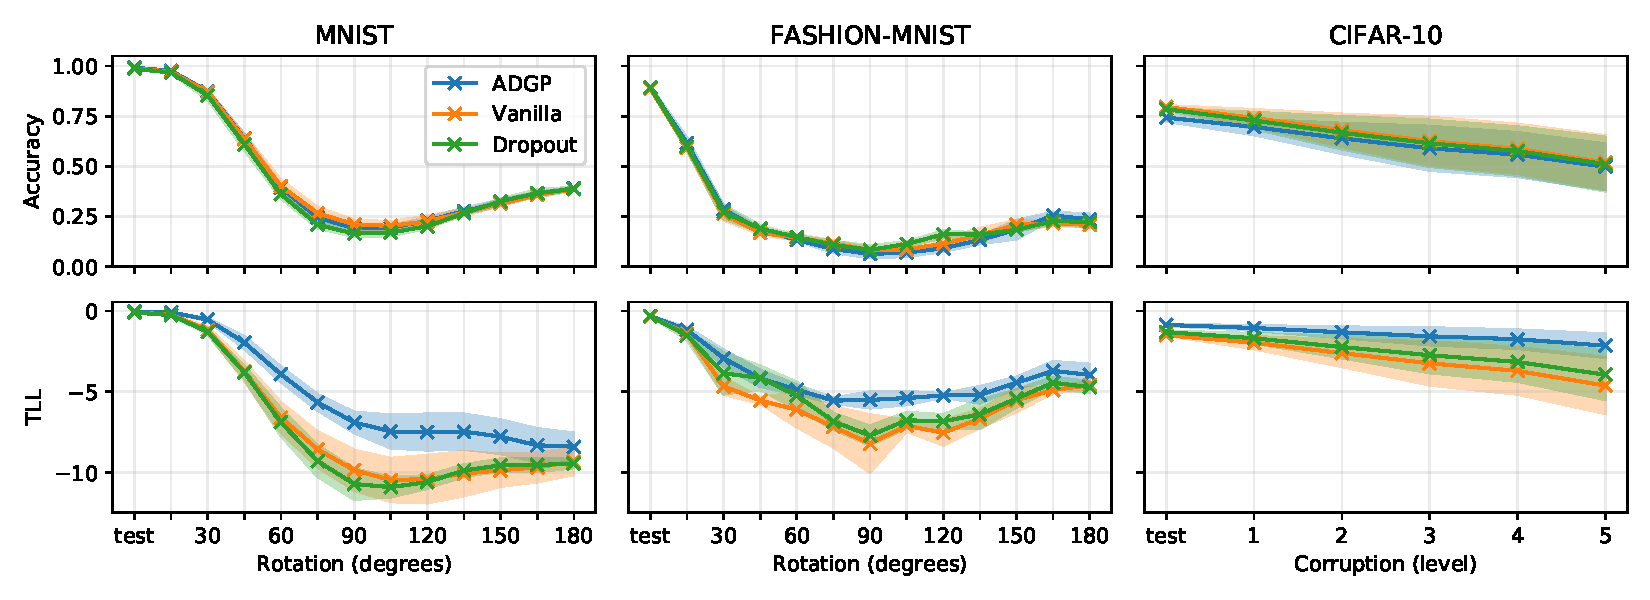
\includegraphics[width=\textwidth]{image_classification}
    \caption{Results on the rotated MNIST, FASHION-MNIST and corrupted CIFAR-10, showing the mean and std. dev. of the accuracy \textbf{(top)}, and test log-likelihood (TLL) \textbf{(bottom)}.}
    \label{fig:image-classification}
\end{figure}

